\section{Anonymous Protocol}\label{sec-protocol}

\begin{figure}[h]
\begin{center}
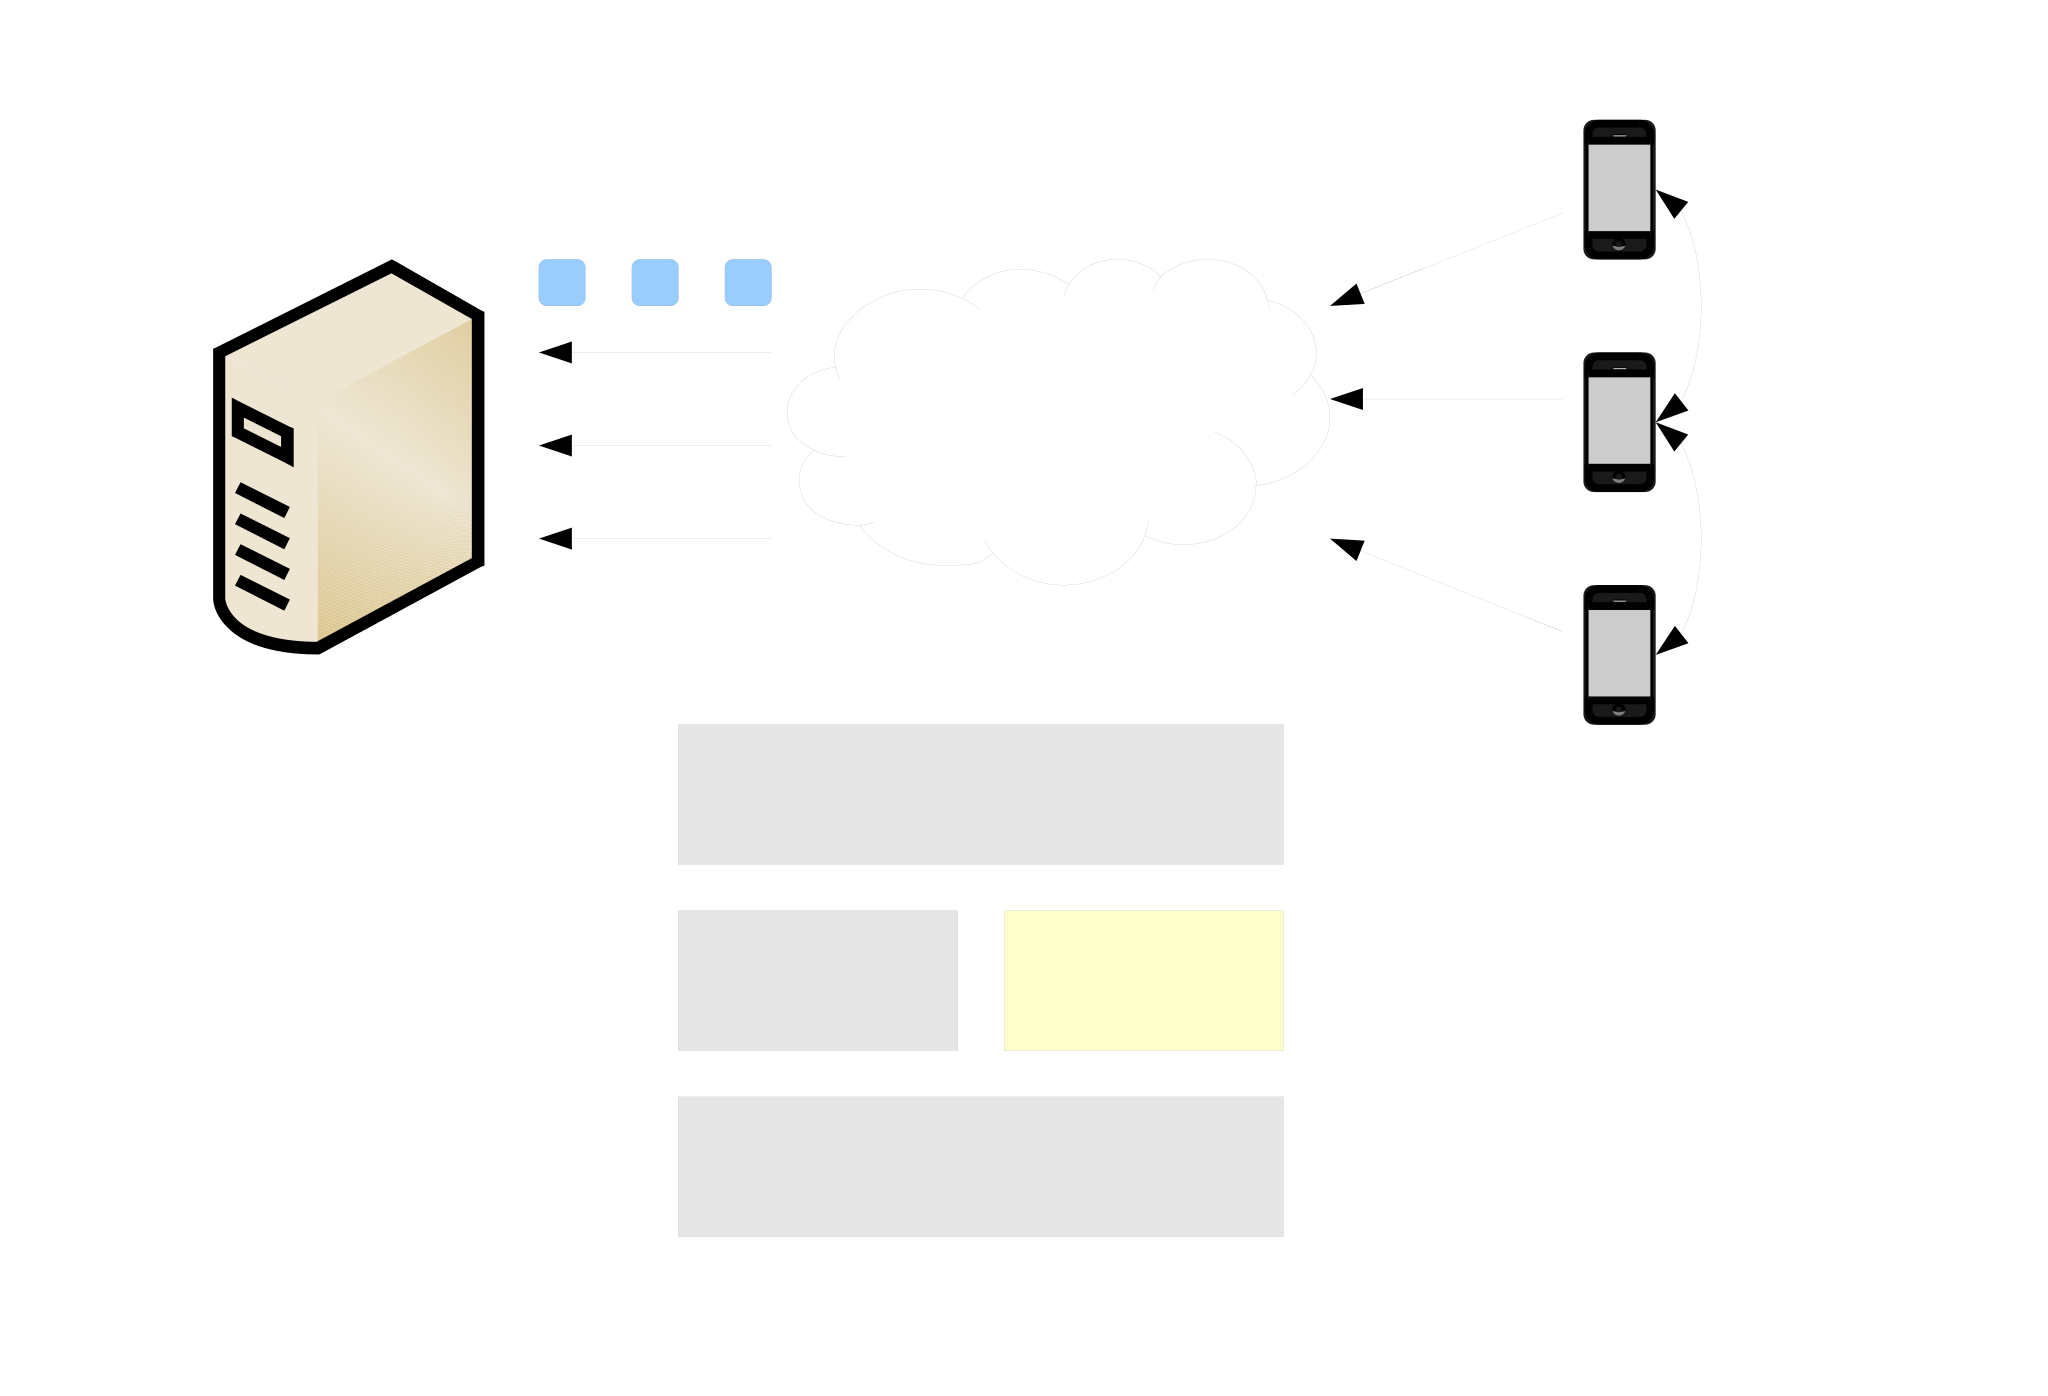
\includegraphics[width=3in]{figure1.eps}
\caption{\small \sl Anonymous Protocol.\label{fig:Stupendous}}
\end{center}
\end{figure}

What we would like is a protocol that completely removes the ownership and
source information from the data transmitted to the data collection server.
Figure 1 illustrates the concept of the theoretical anonymous One-Way
protocol.

We envision the protocol to be a network layer (layer 3) protocol that
replaces the IP protocol. The protocol will be very similar to the IP protocol
in the way that the packets includes the address of the destination host so
that the packets can be correct routed. The protocol should be able to
encapsulate upper layer (e.g. transport layer) data. The only difference is
that each packet does not include the address of the source host. In other
words, contractually, the client does not include the source address and the
server will have no access to the source information and thus keeping the
client's identity private.

Proponents might argue since the protocol resides on network layer (layer 3),
the source address could still be contained in the lower layer, e.g. the link
layer (layer 2). We argue that the source link address is different for
each hop on the route, and a route could easily contain 20 hops; therefore
the probability of tracing the link layer packet back to the original host is
really low.

%\begin{figure}[h]
%\begin{center}
%\includegraphics[width=3in]{arch.eps}
%\caption{\small \sl System Architecture.\label{fig:Stupendous}}
%\end{center}
%\end{figure}

\section{Anonymous Protocol Over Existing Protocols}\label{sec-protocol}
The One-Way protocol introduced in the previous section and Figure 1 is only
a theoretical protocol since it would take significant effort and drastic
change to current networking hardware infrastructure to introduce a new layer 3
routing protocol. In this section we modify the One-Way protocol depicted in
Figure 1 slightly so that it utilizes existing networking infrastructures. We
introduce two modifying approaches: tunneling and One-Way over User Datagram
Protocol (UDP).

\subsection{Tunneling}

In tunneling, the network topology is divided into two parts: a private
network that understands the One-Way protocol and the rest of the world that
only understand the IP protocol. The two parts are connected by the tunnel,
a special device, that does the translation between two routing protocols.

\begin{figure}[h]
\begin{center}
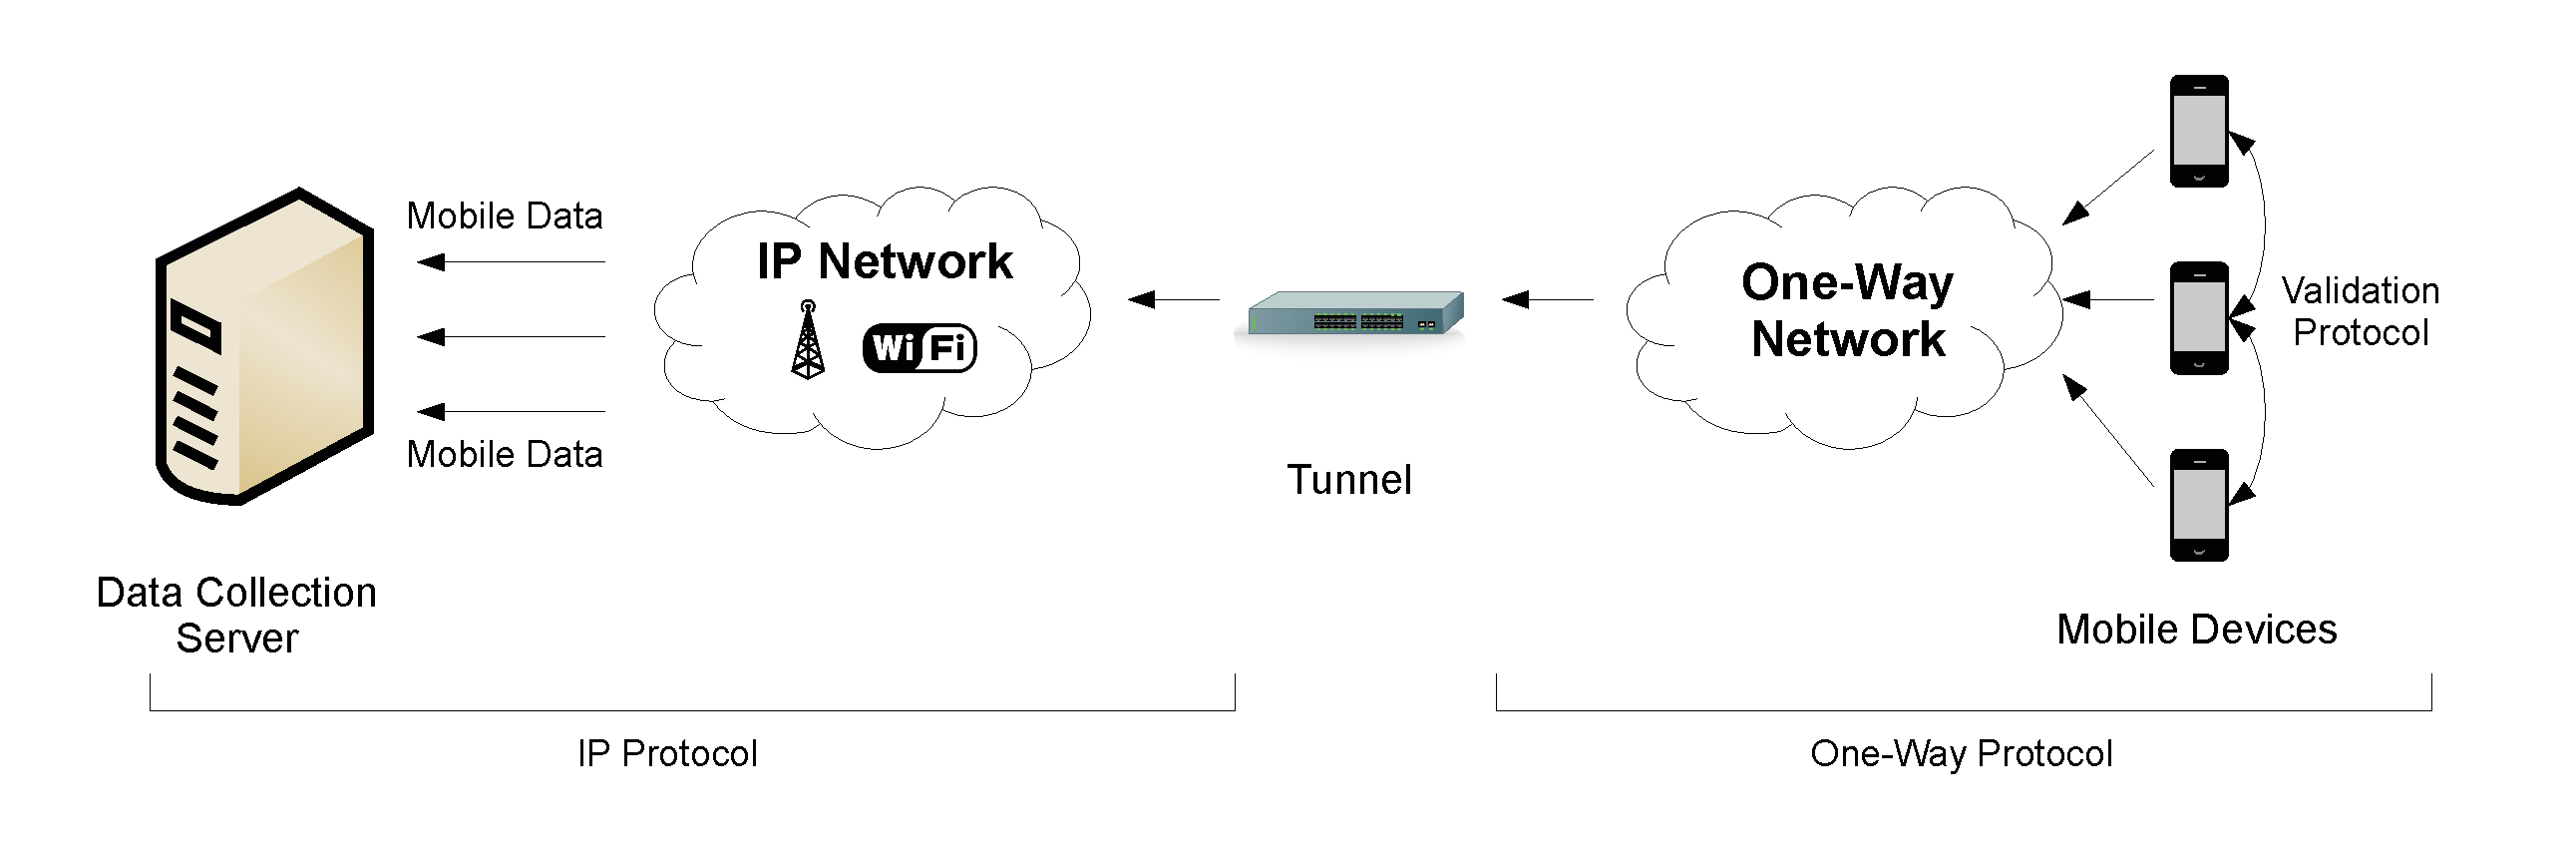
\includegraphics[width=3in]{figure2.eps}
\caption{\small \sl Tunneling.\label{fig:Stupendous}}
\end{center}
\end{figure}

\begin{figure}[h]
\begin{center}
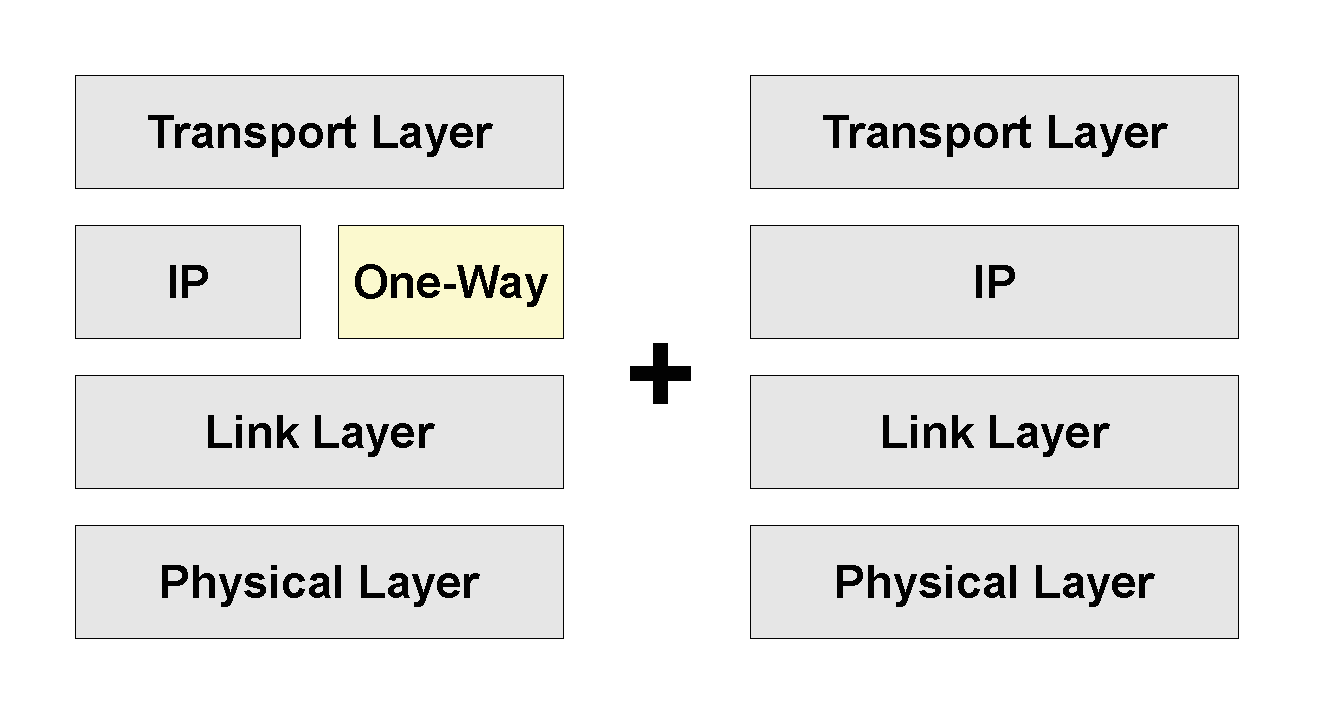
\includegraphics[width=3in]{figure2b.eps}
\caption{\small \sl Tunneling.\label{fig:Stupendous}}
\end{center}
\end{figure}

As illustrated in Figure 2, the tunneling device takes packets from the One-Way
network and forward the
data to the IP network. An important task of the tunneling device is to attach
source IP address to the packets that being forwarded. The device uses it own
IP address as the address of the packets and shields the identity of the mobile
clients. A reason for this tunneling approach is that some internet service
providers (ISP) will block packets without valid source host address. Figure 3
depicts the networking stack configuration of this approach.

Opponent could argument that attacker can still trace the mobile clients to a
specific subnet where the tunneling device resides. We argue that since most of
the clients are highly mobile, and with a number of tunneling device in one
geographic region, the identity of the mobile devices can be protected with high
confidence.

\subsection{Over User Datagram Protocol}
In this approach, we completely do away with a new routing protocol by building
the One-Way protocol as an application layer protocol on top of User Datagram
Protocol (UDP) as illustrated in Figure 4.

\begin{figure}[h]
\begin{center}
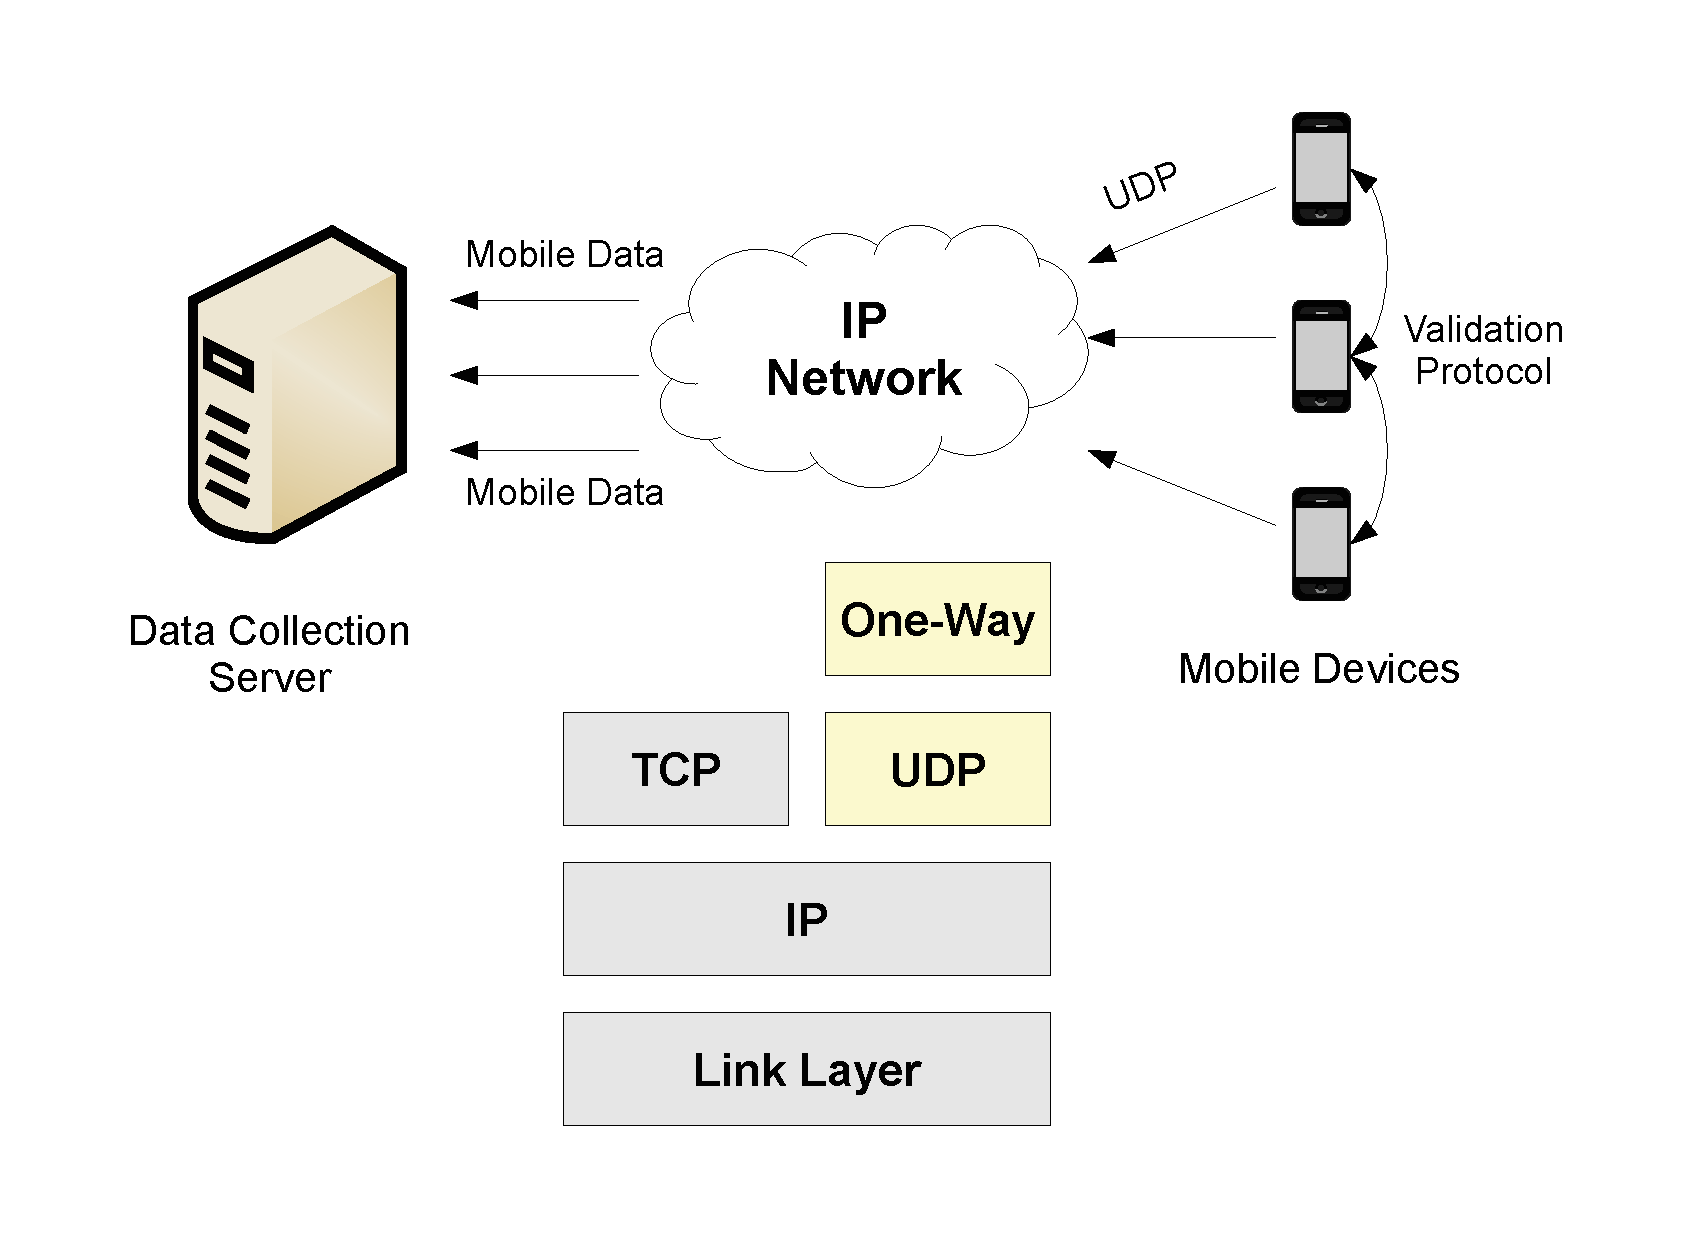
\includegraphics[width=3in]{figure4.eps}
\caption{\small \sl One-Way over UDP.\label{fig:Stupendous}}
\end{center}
\end{figure}

During transmission, the clients divides the data into one or more UDP data packets,
uses arbitrary IP address as the source address -- to protect the identity of the
mobile clients -- and sends the packet into the network.
The reason we use UDP instead of TCP is that since the source IP is arbitrary, TCP
will be unable to establish a connection with the handshaking protocol.

In our experiment, we are able to send IP packets with arbitrary source address into
the network and receive it on the server.

\section{Validation}
This section has not been completed.

\section{Future Work}
Future work includes reliability and security of this approach.

%\begin{enumerate}
%\item
%The client initiates the K-Nearest-Neighbor Query by evaluating
%$k' = k (r + 1)$ where $r$ is the percentage of replication of original
%dataset. The calculation is done on the client side, since only the data owner
%and the client know the value of $r$. Once found, the clients sends $k'$ to the
%service provider.
%\item
%The service provider finds $k'$ records "surrounding" the location of the
%client based on space encryption Hilbert value. For example, if the Hilbert
%value of the client is $H_c$, then the service provider evaluates the query by
%finding Hilbert values of records in the range $[Hc - K'/2, Hc + K'/2]$.
%Service provider returns the $k'$ records to the client as $R$.
%\item
%Due to Hilbert Space Transformation, locations with the closest Hilbert values
%do not necessary have the closest distance in the original space. To compensate,
%after receiving $R$ from the service provider in step 2, the client finds the
%record, $s^*$, with the largest Hilbert distance from itself, calculate the
%physical distance (or range), $d$, to $s^*$, and performs a range query with
%distance of $d$.
%\end{enumerate}



%\begin{figure}[h]
%\begin{center}
%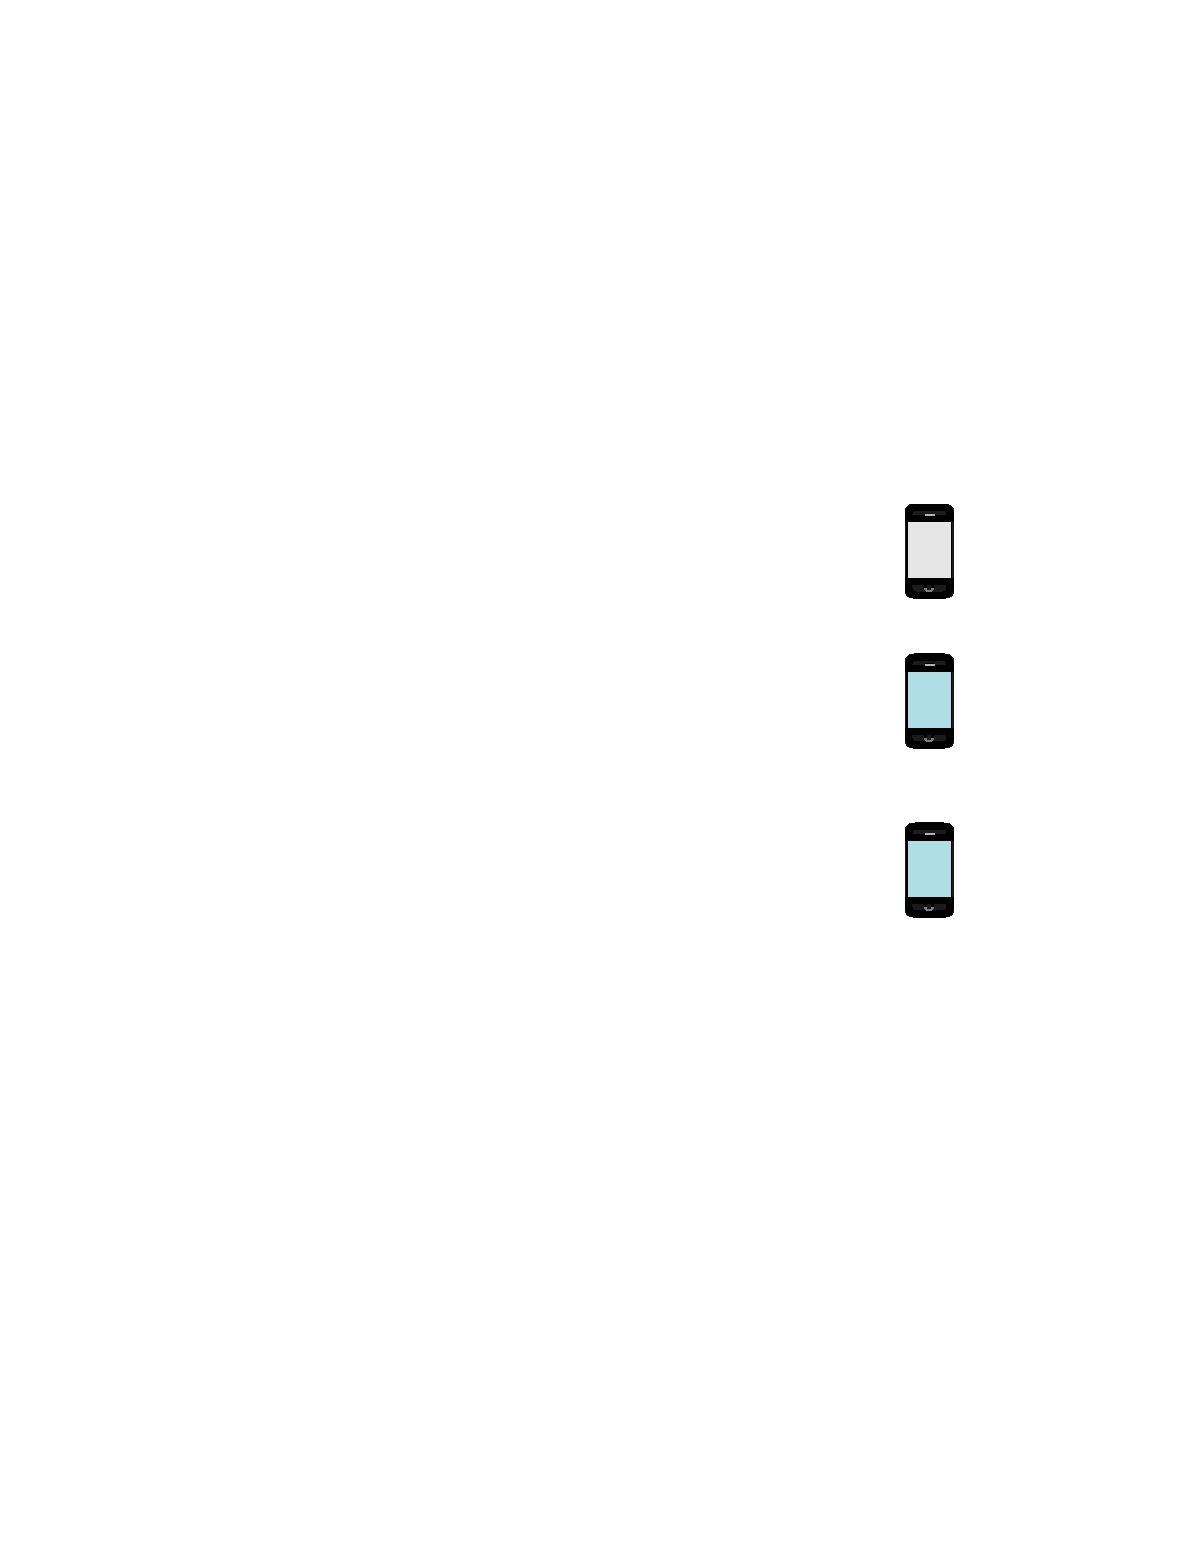
\includegraphics[height=3in]{U1.eps}
%\caption{\small \sl Audit Query Result.\label{fig:Stupendous}}
%\end{center}
%\end{figure}
